\chapter{Трансформер-агностичные модели}\label{ch:tr-ag}
% TODO - ЧТОБЫ ВЕЗДЕ НАЗЫВАЛИСЬ АГНОСТИЧНЫМИ, А НЕ ИНВАРИАНТНЫМИ!!!!
Многозадачные нейросетевые модели, описанные в предыдущем разделе \ref{ch:pseudolabel}, позволяют добиться существенной экономии вычислительных ресурсов. Тем не менее, к числу их неустранимых недостатков относится негибкость. Они поддерживают только один тип голов (multilabel), они требуют наличия меток для каждой задачи у каждого примера. 

В связи с этим была поставлена цель поиска и исследования более эффективных архитектур. В частности, было необходимо предложить многозадачную нейросетевую архитектуру, лишенную описанных выше недостатков архитектуры из \ref{ch:pseudolabel}. Помимо этого, необходимо было исследовать перенос знаний в предложенной нейросетевой архитектуре: как перенос знаний между задачами, так и перенос знаний между языками при использовании многозадачных моделей. При этом задачи для исследования было необходимо выбрать исходя из потребностей реальных диалоговых платформ, например, платформы DREAM\ref{ch:dream}. 

Архитектура, исследование которой проводилось, описана в следующем разделе. Попытки улучшения данной архитектуры описаны отдельно. 

\subsection{Архитектура трансформер-агностичной многозадачной модели}\label{ch:tr-ag:architecture} 
Предложенная многозадачная трансформер-агностичная модель основана на классе \texttt{AutoModel} из HuggingFace, который разрешает использовать разнве модели, основанные на архитектуре Трансформер\footnote{Список поддерживаемых моделей: \url{https://huggingface.co/transformers/v3.0.2/model_doc/auto.html\#automodel}}. Для наших экспериментов, мы использовали модели, основанные на архитектуре типа BERT, но абсолютно тот же подход может применяться и к другим нейросетевым моделям на базе архитектуры Трансформер. 

Этот подход заключается в следующем:
\begin{itemize}

    \item[*] Как и в оригинальной статье~\cite{bert}, возвращаются финальные скрытые состояния для всех токенов и выход пулингового слоя BERT. 

    \item[*] К выходу пулера применяется дропаут, по умолчанию равный 0.2\footnote{Как варьирование dropout, так и варьирование attention dropout не привело к улучшению характеристик модели.}. Для задач выбора из нескольких вариантов ответа или классификации каждого токена в предложении, выход преобразуется аналогично соответствующим задачам. 

    \item[*]После этого этапа, мы применяем задаче-специфичный линейный слой с размерностью выхода \texttt{n}. Для всех задач, кроме регрессии или выбора из нескольких вариантов ответа\footnote{Для задачи выбора из нескольких вариантов ответа, каждой метке изначально относится несколько примеров. Т.е с таким числом классов после преобразования формы число реальных и предсказанных меток соответствует друг другу.}, \texttt{n} равняется числу классов для задачи. Во всех других случаях \texttt{n} равняется 1.
 
    \item[*]В конце применяется функция потерь. Если для каждого примера из задачи ожидается только одна метка, применяется категорическая кросс-энтропия, в остальных случаях - бинарная кросс-энтропия. 

\end{itemize}

Обращу отдельное внимание на то, что в каждом тренировочном батче для данной нейросетевой многозадачной модели должны содержаться примеры только из одной задачи. В противном случае эффективный размер батча для каждой из задач оказывался меньше задаваемого изначально, что приводило к ухудшению метрик модели. 

Такая многозадачная модель почти не требует дополнительных параметров, и, как следствие, дополнительных вычислительных ресурсов(кроме линейных слоев, которые требуют на порядки меньше ресурсов, чем тело архитектуры Трансформер). Так, для моделей типа distilBERT, предложенная многозадачная модель требует всего лишь примерно на  0.1\% больше видеопамяти, чем любая из соответствующих ей однозадачных моделей. В зависимости от числа задач, числа классов и "тела" многозадачной модели, количество дополнительных параметров варьируется вокруг этого числа. 

При этом данная модель является трансформер-агностичной, что позволяет быстро подставлять в нее разные типы базовых моделей. Это выгодно отличает данную модель от иерархических многозадачных моделей, таких, как \cite{PAL:19} и \cite{TaskEmbedded2021}. 

Отдельно выделяю то, что данная модель успешно интегрирована в библиотеку DeepPavlov\cite{Burtsev2018DeepPavlovAO}.

\subsection{Какие эксперименты не сработали}\label{ch:tr-ag:failed_attempts} 
Автор диссертационной работы пробовал большое количество различных вариантов улучшения архитектуры многозадачной трансформер-агностичной модели по сравнению с описанными в разделе \ref{ch:tr-ag:architecture}. 
\begin{itemize} 
 \item[*] Первой серией идей была модификация выхода CLS-выхода модели BERT, который классифицируется задаче-специфичными головами. Для данной задачи проверялось использование задаче-специфичных слоев, описанных в \cite{GhostBERT2021, TaskEmbedded2021, el-nouby2021xcit}. Кроме данных слоев, проверялось также использование LSTM-представления CLS токена или конкатенация этого представления с самим CLS токеном. При проверке на валидационном наборе данных GLUE, прироста средней точности по сравнению с описаннрй выше архитектурой данные эксперименты не дали. 
\item[*] Второй серией идей являлось использование задаче-специфичных тренируемых токенов. А именно, идеи заключались в том, чтобыприсваивать каждой из задач какой-нибудь неиспользуемый токен из словаря BERT (каждой задаче - свой токен). И добавлять этот токен сразу же после CLS к каждой из задач. После чего проводить классификацию не просто по CLS токену, а либо по конкатенации CLS и задаче-специфичного токена, либо же просто по задаче-специфичному токену. На наборе данных GLUE эти идеи не привели к улучшению метрик.

\ю Для случая, когда к каждому примеру добавляется не один задаче-специфичный токен, а сразу все задаче-специфичные токены по очереди (то есть для трехзадачной классификации, условно, каждый пример имеет вид \textit{[CLS] [TOKEN FOR TASK1] [TOKEN FOR TASK2] [TOKEN FOR TASK3] [TOKENIZED_EXAMPLE]}, улучшения при проведении классификации как в предыдущем пункте также не последовало. 

Вероятно, провал этих экспериментов связан с тем, что если CLS-токен был хорошо предобучен на оригинальном BERT для проведения классификации, то задаче-специфичные токены предобучены не были, а какая-то дополнительная полезная информация, зависящая от задачи, через них так и не передавалась(ну или наоборот, она слишком хорошо передавалась через [CLS]. 

\item][*] Хотя исследование разных методов сэмплирования задач при многозадачном обучении не является фокусом данной диссертационной работы, автор также проводил эксперименты и с разными методами сэмплирования. Так, вариант перехода для каждой задачи в режим сходимости (с делением функции потерь для этой задачи на 4),если на ней нет заметного улучшения, и выхода из этого режима, если на этой задаче появляется заметное ухудшение, не сработал. Эксперимент, в котором после некого числа эпох (достаточно большого, чтобы измерить дисперсию модели), модель обучалась только на некой доле самых сложных примеров с самой высокой дисперсией, тоже не сработал\footnote{Справедливости ради, существуют и эффективные способы улучшения сэмплирования, дававшие заметный прирост метрик - например, \cite{GradTS}. Данный подход вполне можно объединить с предлагаемым в моей диссертации.}. 

В числе неудачных экспериментов также можно упомянуть эксперименты по дистилляции более крупных моделей BERT в более мелкие, которые проводились путем добавления в функцию потерь нового члена, "приближающего" веса более крупной модели к соответствующим весам более мелкой (по метрике mean squared error). Эта идея не сработала. Автор предполагает, что это было связано с тем, что данный способ является слишком грубым для того, чтобы приблизиться к адекватной аппроксимации сложных нейросетевых функций, которые используются в модели BERT. В связи ч этим, в дальнейшем идеи с приближением весов не проверялись. 
\subsection{Преимущество трансформер-агностичной многозадачной модели над многозадачной моделью с одним линейным слоем} 
\label{ch:tr-ag:advantages}

Многозадачная трансформер-агностичная модель является логичным усовершенствованием многозадачной модели с одним линейным слоем. По сравнению с данной моделью, многозадачная трансформер-агностичная модель имеет больше гибкости, так как не требует меток для каждой из задач у каждого примера. При этом подобная модель лучше адаптируется к каждой конкретной задаче, так как при обучении на примерах из каждой задачи у этой модели обновляются веса только тех нейронов в финальных линейных, которые отвечают конкретно за эту задачу. В то же время, у модели с одним линейным слоем пример из каждой задачи при обучении чуточку "сбивает" веса \textbf{всех} задач. 

Данный эффект можно сгладить, используя псевдоразметку каждого примера для каждой задачи уже обученными однозадачными моделями, но это требует больших затрат времени и вычислительных мощностей, а также вносит в обучающую выборку для каждой задачи искажения, связанные с необходимостью видеть большое количество не свойственных этой задаче примеров, размеченных каким-то неидеальным образом. Так, для задачи классификации тональности доля положительных обучающих примеров после псевдоразметки, описанной в главе \ref{mtldream:tr-ag}, уменьшилась с 42.4\% до 12.7\% \ref{appendix:sentiment}. При этом все плюсы от псевдоразметки там, где она оправдана, можно получить и при применении многозадачной трансформер-агностичной модели - которая к тому же предоставляет и возможность выбора, на каких задачах делать псевдоразметку, а на каких не делать.

Другое преимущество многозадачной трансформер-агностичной модели, проявляющееся даже на параллельно размеченных данных, заключается в большей гибкости голов. Если модель с одним линейным слоем по факту поддерживает только один тип головы, а имеено multilabel, то многозадачная трансформер-агностичная модель поддерживает и singlelabel головы для каждой задачи. Реальное применение показало, что на тех задачах, где выход модели можно представить в singlelabel виде, его лучше представлять в singlelabel виде. Это, по всей видимости, связано с тем, что задача "выбрать один самый вероятный класс" проще для линейного слоя, чем задача "выбрать сколько-то классов, чья вероятность выше какой-то границы". И применяя трансформер-агностичную модель, мы можем сознательно выбирать решение именно этой задачи.

Еще одно преимущество многозадачной трансформер-агностичной модели, которое в рамках этой работы еще не было раскрыто до конца, заключается в том, что она поддерживает больший спектр задач. В частности, она (в реализации на момент написания диссертационной работы) поддерживает такие задачи, как распознавание именованных сущностей или выбор из нескольких вариантов ответа, которые невозможно реализовать в рамках модели с одним линейным слоем. 


\section{Наборы данных}

Исходя из специфики прикладного применения диалоговой платформы DREAM, было выбрано пять ключевых диалоговых задач для исследования переноса знаний. Это классификация эмоций, классификация токсичности, классификация тональности, классификация интентов и тематическая классификация. Так как одной из задачей диссертационной работы являлось исследование межъязыкового переноса знаний, было подготовлено по два набора данных для каждой из этих задач: русскоязычный и англоязычный набор. Отдельно обращаю внимание, что для классов, одинаковых в русском и английском языке, индексы соответствующих используемых моделью классов были тоже одинаковыми. Размеры каждого из наборов данных по классу и разбиению приведены в Аппендиксе \ref{appendix:tr-ag_sizes}. 

Ниже подробно описаны наборы данных для каждой из диалоговых задач. 

\subsection{Классификация эмоций}
\subsubsection{Англоязычный набор данных} 
В качестве англоязычного набора данных для классификации эмоций, использовался набор данных  \texttt{go\_emotions}~\cite{emotions}. Этот набор данных состоит из коротких комментариев из Реддита \footnote{\url{http://reddit.com}}, таких, как \textit{LOL. Super cute!} или \textit{Yikes. I admire your patience}. Все эмоции из данного набора данных были сгруппированы в семь типов по Экману, а именно \textit{anger}, \textit{fear}, \textit{disgust}, \textit{joy}, \textit{surprise}, \textit{sadness}, и \textit{neutral}. 

После такой группировки, были выбраны только примеры, содержащие только одну метку. Исследование возможностей улучшения классификации таких примеров за счет использования примеров, содержащих более чем одну метку, успехом не увенчалось - подробнее эти попытки описаны в разделе \ref{ch:mtldream:failed_emo_attempts}. 

Примерно 80 процентов данного набора данных, а именно около 39.5 тысяч примеров, составляли тренировочные данные. Размер валидационной выборки примерно равнялся размеру тестовой. 

\subsubsection{Русскоязычный набор данных} 
В качестве русскоязычного набора данных для классификации эмоций, использовался набор данных \texttt{CEDR}~\cite{ru_emotions}\footnote{Набор данных был получен по адресу \url{https://huggingface.co/datasets/cedr}}. Примеры из этого набора могут принадлежать пяти классам - \textit{anger}, \textit{fear}, \textit{joy}, \textit{surprise}, and \textit{sadness}. Помимо этого, примеры из этого набора могут принадлежать более чем одному классу или (в отличие от \texttt{go\_emotions}) не принадлежать ни к какому классу. 

При подготовке набора данных, примеры, которые не принадлежат ни одному классу, были обозначены как принадлежащие классу \textit{neutral}, после чего были выбраны только примеры, принадлежащие одному классу. Соответственно, номенклатура такого набора данных была такая же, как и у англоязычного набора данных, с поправкой на отсутствие класса \textit{disgust}. Впрочем, так как примеров из этого класса и в англоязычном-то наборе данных было меньше, чем 1.5\%, на перенос знкний это сильно не повлияло. 

В оригинальной работе набор данных CEDR ыюбыл разбит только на тренировочную и тестовую выборки в соотношении 80/20. В целях получения полноценной валидационной выборки, 12.5\% тренировочных примеров из CEDR было выделено как валидационный набор данных. Финальный размер тренировочных русскоязычных данных составил около 6.5 тысяч примеров.
 % TODO проверить


\subsection{Классификация тональности}

\subsubsection{Англоязычные данные} 
В качестве англоязычного набора данных для классификации тональности, использовался набор данных \texttt{DynaSent}(r1)~\cite{sentiment} for the sentiment classification. Чтобы не переусложнять набор данных по сравнению с русскоязычными данными, использовались только примеры из первого этапа сбора данных DynaSent. В данном наборе данных есть 80.5 тренировочных примеров, разделенных на три класса - positive, negative, neutral. 

\subsubsection{Русскоязычные данные} 
В качестве русскоязычного набора данных для классификации тональности, использовался набор данных \texttt{RuReviews}~\cite{ru_sentiment}. Данный набор данных содержит отзывы из крупного российского электронного магазина из категории "Женские товары и ассексуары". Данный набор данных был выбран, потому что он имеет достаточно большой размер(82.6 тысяч тренировочных примеров) и находится в открытом доступе, несмотря на свою специфичность. Так как авторы набора данных не предоставили его разбиение на тренировочные, валидационные и тестовые данные, он был разбит на эти три категории в тех же пропорциях, что и у набора данных
 \texttt{DynaSent}(r1). 

\subsection{Классификация токсичности}
\subsubsection{Русскоязычный датасет} 
Для английского языка в работе использовался набор данных  \texttt{Wiki Talk}~\cite{toxic} для задачи классификации токсичности. В этом наборе данных, состоящем из комментариев из Википедии и имевшем примерно 127.6 тысяч тренировочных примеров, есть всего два класса: \textit{toxic} и \textit{not toxic}. К первому классу относится примерно 10 процентов примеров (часть из которых слишком неблагозвучна для того, чтобы приводить их в диссертации). Ко второму классу, соответственно, примерно 90 процентов.  В работе использовалась предобработанная версия набора данных, предоставленная HuggingFace\footnote{\url{https://huggingface.co/datasets/OxAISH-AL-LLM/wiki_toxic}}. Данная версия подверглась незначительной очистке - к примеру, если какая фраза начиналась и заканчивалась с кавычек, эти кавычки удалялись.  
%CHECK SIZES
\subsubsection{Англоязычный датасет}
Для русского языка в работе использовался двухклассовый набор данных \texttt{RuToxic} ~\cite{ru_toxic}. Этот набор данных состоял из комментариев из Двача, крупнейшего русскоязычного анонимного форума \footnote{\url{http://2ch.hk}}. Набор данных состоит из примерно 162 тысяч примеров, примерно 31 тысяча из которых - токсичные. Так как авторы не предоставили оригинальное разбиение данных в своем репозитории\footnote{Ссылка на репозиторий: \url{https://github.com/s-nlp/rudetoxifier}}, датасет был разбит на тренировочную, валидационную и тестовую выборку в тех же пропорциях, что и англоязычный датасет. Итоговая тренировочная выборка содержала примерно 93.3 тысячи примеров. 

\subsection{Классификация интентов и тематическая классификация }
%TODO. Набор данных - - датасет? Топик - тема? Единообразно сделать
Мы использовали набор данных \texttt{MASSIVE}~\cite{massive} для классификации интентов и для тематической классификации как для русского, так и для английского языка. Этот набор данных основан на англоязычном наборе данных SLURP\cite{clurp}, содержащем фразы, предназначенные голосовому ассистенту. 
 Все примеры из этого набора данных были одновременно размечены(с адаптацией под национальные особенности) для 51 языка, включая русский и английский. Этот набор данных содержит для каждого языка 11514 тренировочных примера, 2033 валидационных примера и 2974 тестовых примера. Каждый пример принадлежит одному из 60 интентов и одной из 18 тем. 

Для каждой задачи, число примеров для каждого класса в тренировочных, валидационных и тестовых данных приведено в Аппендиксе \ref{appendix:sizes_tr-ag} 
% TODO. Как смотрится ссылка? 

\section {Настройки экспериментов}
%TODO. Беты единообразно
%TODO. Почему не тюним скорость обучения? Васю спросить о ссылке на статью
Для всех описанных в данной статье экспериментов, автор работы использовал оптимизатор AdamW~\cite{adam} с  $\beta_1$=0.9, $\beta_2$=0.99 и начальной скоростью обучения 2e-5. В качестве метрики, определяющей остановку обучения, использовалась средняя точность для всех задач\footnote{Или точность для одной задачи, если модели обучались в однозадачном режиме.}. Если на валидационных данных средняя точность не росла в течение двух эпох подряд, скорость обучения уменьшалась в два раза. Если на валидационных данных средняя точность не росла в течение трех эпох подряд, обучение прекращалось. В качестве итоговой версии модели, выбиралась модель с наилучшей средней точностью на валидационных данных. 

Как правило, обучение завершалось в течение менее, чем 10-15 эпох, и всегда - в течение менее, чем 25 эпох. 

Размер батча при тренировке моделей был выбран равным 160 для того, чтобы максимально быстро проводить серии экспериментов на доступных в рамках Лаборатории нейронных сетей и глубокого обучения МФТИ вычислительных мощностях - видеокартах Nvidia GeForce 1080 Ti и Tesla A100. 
%TODO названия видеокарт
При обучении, примеры для каждой задачи выбрались с вероятностью, пропорциональной размеру её набора данных. Ниже подобный способ выбора примеров будет обозначаться как простое сэмплирование. Были также проведены предварительные эксперименты(на русскоязычных и англоязычных дистиллированных моделях, на полной обучающей выборке) с выбором других способов сэмплирования: а именно однородного (с одинаковой вероятностью выбора примера для каждой из задач) и аннеализованное(описанное в \cite{PAL:19}). Данные эксперименты не показали стойкого улучшения показателей по сравнению с простым сэмплированием, поэтому использовалось именно оно. 

Результаты всех экспериментов на диалоговых данных были усреднены по 3-5 запускам\footnote{ Для каждого из таких запусков, отличалась инициализация задаче-специфичных слоев и параметр random seed при сэмплировании.}. Подробные результаты для каждого запуска приведены в Аппендиксе \ref{appendix:tr-ag:allruns}. 

\section{Многозадачные и однозадачные модели - эксперименты на полном наборе данных} 
% TODO BACKBONE ВИДЕОПАМЯТЬ ТЕРМИНЫ
Для английского языка, проводились эксперименты на трех разных базовых моделях типа BERT: \textit{distilbert-base-cased}~\cite{alina}, \textit{bert-base-cased}, И \textit{bert-large-cased}~\cite{bert}.  Эти три модели существенно различаются по объему потребляемых вычислительных ресурсов. Так, 
\textit{distilbert-base-cased} требует на 40\% меньше видеопамяти, чем \textit{bert-base-cased}, а \textit{bert-large-cased} требуетзанимает в  3.1 раза больше видеопамяти, чем \textit{bert-base-cased}. Таким образом, эти три базовые модели покрывают большое количество разных способов использования нейросетевых классификаторов для диалоговых моделей. 

Для русского языка, эксперименты проводились с базовыми моделями \textit{DeepPavlov/distilrubert-base-cased-conversational}~\cite{distilrubert} and \textit{DeepPavlov/rubert-base-cased-conversational}~\cite{rubert}.

Результаты экспериментов на описанных выше диалоговых данных для англоязычных и русскоязычных моделей приведены в Таблице \ref{tab:tr-ag:en_results} и Таблице \ref{tab:tr-ag:ru_results} соответственно. Для каждого эксперимента, приведена точность и усредненное macro-f1.
% TODO Average F1 macro? Как говорится? 

Другой важной исследовательской задачей является оценка многозадачной трансформер-агностичной модели на других типах задач и данных, отличающихся от приведенных выше. В целях решения данной задачи, автор также провел аналогичные эксперименты для англоязычных моделей на бенчмарке GLUE\cite{GLUE:19} с теми же самыми гиперпараметрами \footnote{В связи с тем, что результаты на бенчмарке GLUE оценивается на сервере, у которого есть жесткие ограничения на то, сколько раз подряд можно отправлять свои результаты, усреднение по нескольким запускам на бенчмарке GLUE не проводилось.}. Результаты этих экспериментов представлены в таблице \ref{tab:tr-ag:glue} .

Для всех таблиц в этой главе Acc означает точность, F1 метрику F1, режим S означает отдельную модель для каждую из задач и режим M многозадачную модель. "Число батчей" означает число батчей, которые видела модель при своем обучении.

\begin{table*}
 \caption{Метрики англоязычных моделей (точность/f1 macro) для пяти англоязычных диалоговых задач.Режим S означает однозадачные модели, режим M означает многозадачные модели. Усреднено по трем запускам.}
 \label{tab:tr-ag:en_results}
\centering
\resizebox{\textwidth}{!}{%
\begin{tabular}{c|c|c|c|c|c|c|c|c}
\hline
\multirow{2}{*}{Модель} & \multirow{2}{*}{Режим} & \multirow{2}{*}{Среднее} & Эмоции & Тональность & Токсичность & Интенты & Темы & Число \\
& & & 39.4k & 80.5k & 127.6k & 11.5k & 11.5k & батчей \\ \hline
\textit{\multirow{2}{*}{distilbert-base-cased}} & S & \textbf{82.9/78.4} & \textbf{70.3/63.1} & 74.7/74.3 & 91.5/81.2 & \textbf{87.4/82.7} & \textbf{91.0/90.6} & 11390 \\
 & M  & 82.1/77.2 & 67.7/60.7 & \textbf{75.2/75.0} & 90.6/79.8 & 86.3/80.4 & 90.8/90.1 & 14000 \\ \hline
\textit{\multirow{2}{*}{bert-base-cased}} & S & \textbf{83.9/79.7} & \textbf{71.2/64.2} & 76.1/75.8 & \textbf{93.2/83.5} & \textbf{87.9/84.2} & \textbf{91.3/90.7} & 9470 \\
 & M &  83.0/78.4 & 69.0/63.1 & \textbf{76.5/76.4} & 91.4/80.8 & 87.1/81.2 & 91.2/90.6 & 11760 \\ \hline
\textit{\multirow{2}{*}{bert-large-cased}} & S &  \textbf{84.7/80.5} & \textbf{70.9/64.4} & \textbf{80.5/80.4} & \textbf{92.1/82.2} & \textbf{88.4/84.9} & 91.3/90.7 & 8526 \\
 & M  & 83.6/78.7 & 69.0/61.8 & 79.0/78.9 & 91.3/80.9 & 87.3/80.9 & \textbf{91.3/90.8} & 11200 \\ \hline
 \end{tabular}
 }
 
begin{table*}
 \caption{Метрики русскоязычных моделей(точность/f1 macro) для пяти диалоговых задач. Режим S означает однозадачные модели, режим M означает многозадачные модели. Усреднено по трем запускам.}
 \label{tab:tr-ag:ru_results}
\centering
\resizebox{\textwidth}{!}{%
\begin{tabular}{c|c|c|c|c|c|c|c|c}
\hline
\multirow{2}{*}{Модель} & \multirow{2}{*}{Режим} & \multirow{2}{*}{Среднее} & Эмоции & Тональность & Токсичность & Интенты & Темы & Число \\
& & & 6.5k & 82.6k & 93.3k & 11.5k & 11.5k & батчей \\ \hline
\textit{DeepPavlov/distilrubert-base-cased-conversational} & S & 86.9/84.1 & 82.2/76.1 & 77.9/78.2 & 97.1/95.4 & 86.7/81.6 & 90.4/89.5 & 8472 \\ \hline
\textit{DeepPavlov/distilrubert-base-cased-conversational} & M & 86.3/82.6 & 81.0/74.6 & 77.7/77.7 & 96.9/95.0 & 85.2/75.9 & 90.7/89.9 & 8540 \\ \hline
\textit{DeepPavlov/rubert-base-cased-conversational} & S & 86.5/83.4 & 80.9/75.3 & 78.0/78.2 & 97.2/95.6 & 86.2/79.1 & 90.0/89.0 & 7999 \\ \hline
\textit{DeepPavlov/rubert-base-cased-conversational} & M & 86.2/82.6 & 80.5/73.8 & 77.6/77.6 & 96.8/95.0 & 85.3/76.9 & 90.5/89.8 & 8113 \\ \hline
 \end{tabular}
 }

\begin{table*}
\caption{Метрики многозадачной трансформер-агностичной модели для набора задач GLUE. M.Corr означает корреляцию Мэттью, P/S означает корреляцию Пирсона-Спирмена, Acc точность, F1 - f1 метрику. Режим S означает однозадачные модели, режим M означает многозадачные модели. Размер означает размер тренировочного набора данных}
\label{tab:tr-ag:mtl_glue}
\centering
\resizebox{\textwidth}{!}{%
\begin{tabular}{c|c|c|c|c|c|c|c|c|c|c|c|c}
\hline
\multirow{3}{*}{Модель} & \multirow{3}{*}{Режим}  & Среднее & CoLA & SST-2 & MRPC &STS-B &QQP&MNLI & QNLI & RTE & AX & Число \\
       &        & Размер  & 8.6k & 67.3k & 2.5k & 5.7k & 363.8k & 392.7k & 104.7k & 2.5k & как у MNLI & батчей \\ 
       &        & метрика  & M.Corr & Acc & F1/Acc & P/S Corr & F1/Acc & Acc(m/mm) & Acc & Acc & M.Corr &  \\ \hline
Человек & - & 87.1 & 66.4 & 97.8 & 86.3/80.8 & 92.7/92.6 & 59.5/80.4 & 92.0/92.8 & 91.2 & 93.6 & - & -\\ \hline
%\textit{\multirow{2}{*}{distilbert-base-cased}} & S & 73.1 & \textbf{42.4} & \textbf{92.1} & 85.6/\textbf{80.3} & 78.8/76.8 & \textbf{69.5/88.5} & \textbf{81.3/80.8} & \textbf{87.5} & 49.8 & 29.9 & 70846 \\ 
\textit{\multirow{2}{*}{distilbert-base-cased}} & S & 73.3 & \textbf{42.4} & \textbf{92.1} & 85.6/\textbf{80.3} & 78.8/76.8 & \textbf{69.5/88.5} & \textbf{81.3/80.8} & \textbf{87.5} & 52.1 & 29.9 & 70861 \\ 
 & M & \textbf{74.5} & 36.0 & 91.0 & \textbf{85.7}/79.9 & \textbf{82.6/81.6} & 68.4/87.4 & 80.4/80.3 & 86.0 & \textbf{69.5} & \textbf{30.1} & 88905 \\  \hline
\textit{\multirow{2}{*}{bert-base-cased}} & S & 77.3 & \textbf{53.7} & \textbf{93.2} & \textbf{87.7/82.8} & 83.8/82.2 & \textbf{70.3/88.9} & \textbf{83.8/83.1} & \textbf{90.6} & 62.1 & 32.1 & 42722\\ 
 & M & \textbf{77.8} & 45.8 & 92.9 & 86.8/82.2 & \textbf{85.3/84.7} & 70.2/88.6 & 83.5/82.6 & 90.1 & \textbf{74.5} & \textbf{32.8} & 112613\\  \hline
\textit{\multirow{2}{*}{bert-large-cased}} & S & \textbf{79.5} & \textbf{59.2} & \textbf{94.9} & 85.0/80.6 & \textbf{85.8/84.5} & 70.5/89.1 & \textbf{86.7/85.6} & 92.2 & 70.1 & \textbf{39.4} & 37290 \\ 
 & M & \textbf{79.5} & 50.8 & 94.1 & \textbf{87.3/82.8} & 83.8/83.9 & \textbf{71.0/89.2} & 85.9/85.0 & \textbf{92.4} & \textbf{78.5} & 38.5 & 53343 \\  \hline
\end{tabular}
}
\end{table*}

В общем и целом, метрики многозадачных трансформер-агностичных моделей на диалоговых как для русского, так и для английского языка примерно соответствуют метрикам однозадачных моделей. 
 Для бенчмарка GLUE многозадачные модели дпже превосходят по своей средней метрике однозадачные модели за счет малоразмерных задач (STS-B, AX и особенно RTE), на которых лучше работает перенос знаний с задач, у которых более крупная обучающая выборка. 

Среди поставленных в работе задач было также исследование того, как будет меняться эффект переноса знаний при уменьшении размера обучающей выборки. Данному исследованию посвящен следующий раздел. 

\subsection{Эффект уменьшения размера обучающей выборки (англоязычные данные)}
% TODO - Автор делал или в пассивном залоге? Как писать? 
В работе был также исследован эффект уменьшения размера обучающей выборки для англоязычных данных. В частности, автор работы обучал модель с теми же гиперпараметрами, что и в предыдущем режиме, но только на небольшой доле тренировочных данных. При этом валидационные и тестовые данные, для чистоты эксперимента, не менялись. В связи с малым размером обучающей выборки, для этого эксперимента данные усреднялись по пяти запускам. Для ускорения вычислений, эксперименты в этом разделе проводились только для базовой модели \textit{distilbert-base-cased}. 

Особо отмечаю, что для каждого такого эксперимента разбиение было одним и тем же, то есть при проведении любого эксперимента с тем или иным процентом тренировочных данных в этих данных содержались данные из всех экспериментов с меньшими процентами тренировочных данных. 

Результаты данного эксперимента представлены в Таблице ~\ref{tab:tr-ag:en_dialog_part} и на Графике \ref{fig:tr-ag:en_dialog_part}.

Из представленных данных можно увидеть, что в общем и целом, многозадачный перенос знаний работает лучше для задач с меньшим числом примеров (при условии, что в обучающей выборке есть задачи, у которых число примеров существенно больше). 

В общем и целом, можно сделать вывод, что метрики многозадачных моделей превосходят метрики для однозадачных моделей только на небольших данных -(2-5\% от всего набора англоязычных данных), и уже на 9\% от набора англоязычных данных это преимущество исчезает. Более подробно результаты этого эксперимента проанализированы в разделе \ref{tr-ag:discussion_conclusion}

\begin{figure}
\centering
\caption{Average accuracy for the five dialog tasks. Impact of reducing training data. Averaged by five runs.}
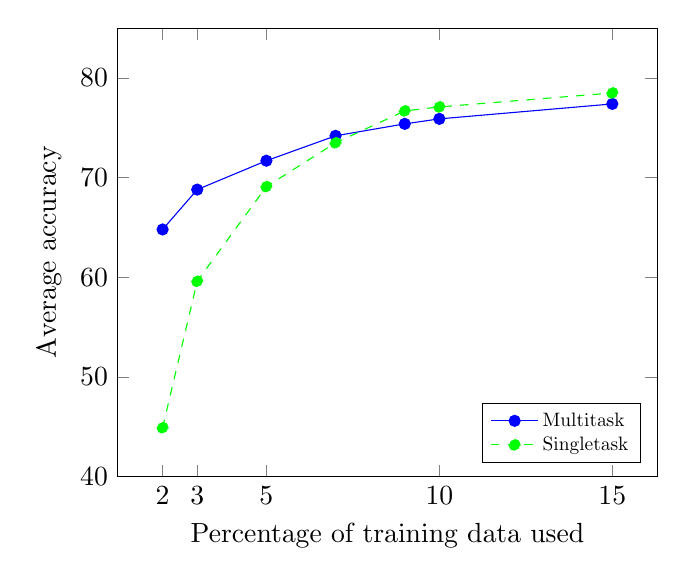
\begin{tikzpicture}
\label{fig:mtl_dialog_part}
\begin{axis}[xlabel = Percentage of training data used,
ylabel = Average accuracy,
legend pos= south east,
% width=10cm,
% height=10cm,
% xmin=2,
% xmax=100,
xtick={2,3,5,10,15},
ymin=40,ymax=85,
legend cell align={left},
legend style={nodes={scale=0.7, transform shape}}
]
\addplot[color=blue,solid, mark=*] coordinates {
(2, 64.8)%50
(3, 68.8)%50
(5, 71.7)%100
(7,74.2)
%(7.5,74.6)
% (8,74.9)
(9,75.4)
(10, 75.9)%300
(15, 77.4)
};
\addlegendentry{Multitask}
\addplot[color=green,dashed,mark=*] coordinates {
(2, 44.9)%50
(3, 59.6)%100
(5, 69.1)%300
(7,73.5)
%(7.5,73.5)
% (8,73.8)%500
(9,76.7)
(10,77.1)
(15, 78.5)
};
\addlegendentry{Singletask}
\end{axis}%
\end{tikzpicture}%
\end{figure}

 
 %TODO - Italicize all backbones? 
\end{table*}
\begin{table*}
\caption{Точность/ F1.  Режим M означает многозадачные модели, режим S означает однозадачные модели, и Доля означает долю использованных тренировочных данных. Базовая модель distilbert. Усреднено по пяти запускам. }
\label{tab:mtl_dialog_part}
\resizebox{\textwidth}{!}{%
\begin{tabular}{c|c|c|c|c|c|c|c|c}
\hline
 \multirow{2}{*}{Режим} &  \multirow{2}{*}{Доля} &  \\multirow{2}{*}{Среднее} & Эмоции & Тональность & Токсичность & Интенты & Темы & Число \\
& & & 39.4k & 80.5k & 127.6k & 11.5k & 11.5k & seen \\
\hline 
S & 15\% & 78.5/70.9 & 65.8/50.6 & 69.3/68.8 & 92.2/81.2 & 78.7/68.8 & 86.3/85.1 & 2173 \\ \hline
M & 15\% & 77.4/70.6 & 64.0/55.0 & 68.3/67.7 & 91.6/80.0 & 76.9/64.6 & 86.4/85.4 & 4741 \\ \hline
S & 10\% & 77.1/68.4 & 64.6/45.0 & 68.3/67.8 & 92.2/81.0 & 75.5/64.7 & 84.8/83.3 & 1579 \\ \hline
M & 10\% & 75.9/69.1 & 62.6/53.6 & 66.6/65.8 & 91.5/79.7 & 74.3/63.2 & 84.6/83.3 & 4295 \\ \hline
S & 9\% & 76.7/67.4 & 64.6/43.9 & 68.2/67.7 & 91.8/80.4 & 74.4/62.7 & 84.2/82.4 & 1457 \\ \hline
M & 9\% & 75.4/67.8 & 62.1/52.4 & 66.5/65.7 & 91.4/79.5 & 72.4/58.5 & 84.4/83.0 & 3695 \\ \hline
%S & 8\% & 73.8/64.6 & 63.7/43.5 & 67.6/67.0 & 92.0/80.5 & 62.0/49.7 & 83.9/82.1 & 1381 \\ \hline
%M & 8\% & 74.9/67.2 & 61.7/51.4 & 66.7/66.0 & 91.5/79.5 & 71.1/57.3 & 83.6/81.7 & 3511 \\ \hline
%S & 7.5\% & 73.5/64.0 & 63.8/42.5 & 67.4/66.9 & 91.6/80.1 & 61.3/48.6 & 83.6/81.7 & 1293 \\ \hline
%M & 7.5\% & 74.6/66.9 & 61.0/50.2 & 67.0/66.4 & 91.5/79.5 & 70.3/56.9 & 83.2/81.4 & 2995 \\ \hline
S & 7\% & 73.5/64.0 & 63.3/42.1 & 67.9/67.4 & 91.8/80.1 & 61.4/49.4 & 83.3/81.1 & 1251 \\ \hline
M & 7\% & 74.2/66.4 & 61.1/50.4 & 65.8/65.1 & 91.0/78.9 & 70.0/56.3 & 83.1/81.3 & 2882 \\ \hline
S & 5\% & 69.1/59.0 & 62.5/38.9 & 66.9/66.3 & 91.8/79.9 & 42.7/30.8 & 81.6/78.8 & 901 \\ \hline
M & 5\% & 71.7/62.4 & 60.5/48.6 & 64.4/63.4 & 90.8/78.5 & 62.4/44.4 & 80.2/77.3 & 2381 \\ \hline
S & 3\% & 59.6/49.0 & 60.6/37.7 & 65.2/64.5 & 91.8/79.3 & 26.5/16.9 & 54.0/46.5 & 584 \\ \hline
M & 3\% & 68.8/58.1 & 58.6/42.7 & 62.5/61.3 & 91.0/78.3 & 55.5/37.1 & 76.4/71.0 & 1566 \\ \hline
S & 2\% & 44.9/31.5 & 48.7/21.7 & 39.6/26.5 & 91.8/79.0 & 2.6/0.2 & 41.4/30.1 & 274 \\ \hline
M & 2\% & 64.8/52.1 & 57.6/38.4 & 61.4/60.1 & 90.8/78.0 & 44.2/23.5 & 69.9/60.4 & 923 \\ \hline
\end{tabular}
}
\end{table*}


Другим интересным направлением исследований является исследование переноса знаний между английским и русским языками в многозадачных моделях. Для исследования данного переноса автор диссертационной работы использовал мультиязыковые базовые модели, предобучавшиеся на большом числе языков. 


\subsection{Многоязычные многозадачные модели - эффект кросс-языкового обучения}

На этой стадии экспериментов, использовались только многоязычные модели. В качестве многоязычных базовых моделей использовались \textit{distilbert-base-multilingual-cased} и \textit{bert-base-multilingual-cased}. На этом этапе решались следующие задачи:

 \begin{itemize}
\item[*] Сравнить качество многозадачных и однозадачных моделей для русского языка при использовании многоязычных базовых моделей. 
\item[*] Проверить, как меняются результаты у однозадачных и у многозадачных моделей, если добавлять при их обучении к русскоязычным данным англоязычные данные, объединяя данные по задаче(то есть для каждой задачи, учить модель на английских и русских данных, но валидировать только на русских). 
\item[*] Проверить, дает ли для описанного в предыдущем пункте какое-то улучшение, если считать англоязычные задачи отдельными задачами (валидируясь все так же только на русскоязычные данных), и соответственно, при обучении на русскоязычных задачах использовать только русскоязычные данные, а при англоязычных - только англоязычные. 
\end{itemize} 

Заметим, что так как англоязычных открытых данных для большинства задач гораздо больше, чем русскоязычных, именно изучение переноса знаний с английского языка на русский представляет бОльший практический интерес, чем изучение переноса знаний с русского языка на английский. Хотя в разделе \ref{ch:yaqtopics} изучается и такой перенос знаний тоже. 
%TODO. Формат представления Accuracy /f1 - должен быть единообразным по диссеру? 
%TODO. Выделять режимы экспериментов в таблицах и перед ними через Italic? 
\begin{table*}
\caption{Точность/f1 macro на русскоязычных данных для многоязычных моделей. Режим S означает однозадачные модели, режим M - многозадачные модели. RU означает русскоязычные данные , EN означает англоязычные данные. Объединенные означает, что русскоязычные и англоязычные данные объединены по задаче, Отдельные означает, что русскоязычные и англоязычными задачи считаются отдельными задачами. Усреднено по трем запускам. }
\label{mult_results}
%\begin{tabular}{|c|c|c||c|c|c|c|c|c|} \hline
\scalebox{0.8}{
\begin{tabular}{|c|c|c||c|c|c|c|c|c||c|} \hline
Модель & \begin{tabular}[c]{@{}l@{}}Тренировочные\\данные\end{tabular} & Режим & Среднее & \begin{tabular}[c]{@{}l@{}}Эмоции\end{tabular} & \begin{tabular}[c]{@{}l@{}}Тональность\end{tabular} & \begin{tabular}[c]{@{}l@{}}Токсичность\end{tabular} & \begin{tabular}[c]{@{}l@{}}Интенты\end{tabular} & \begin{tabular}[c]{@{}l@{}}Темы\end{tabular} &\begin{tabular}[c]{@{}l@{}}Число\\батчей\end{tabular} \\
\hline \hline
\textit{distilbert-base-multilingual-cased} & RU & S & 84.7/81.0 & 77.4/69.1 & 77.7/77.9 & 96.7/94.8 & 83.5/76.6 & 88.1/86.9 & 10058 \\ \hline
\textit{distilbert-base-multilingual-cased} & RU & M & 84.3/80.2 & 78.1/70.5 & 76.8/76.7 & 96.5/94.4 & 81.9/72.3 & 88.2/87.1 & 9821 \\ \hline
\textit{distilbert-base-multilingual-cased} & \begin{tabular}[c]{@{}l@{}}RU+EN,\\объединенные\end{tabular} & S & 85.2/81.8 & 78.9/70.2 & 77.4/77.3 & 96.8/94.9 & 84.7/79.1 & 88.4/87.4 & 31843 \\ \hline
\textit{distilbert-base-multilingual-cased} & \begin{tabular}[c]{@{}l@{}}RU+EN,\\объединенные\end{tabular} & M & 84.5/81.1 & 77.9/70.7 & 76.6/76.7 & 96.5/94.5 & 82.9/76.5 & 88.4/87.2 & 17790 \\ \hline
\textit{distilbert-base-multilingual-cased} & \begin{tabular}[c]{@{}l@{}}RU+EN,\\отдельные\end{tabular} & M & 84.4/80.6 & 77.6/70.0 & 76.8/77.1 & 96.5/94.5 & 82.4/73.9 & 88.3/87.2 & 23688 \\ \hline
\textit{bert-base-multilingual-cased} & RU & S & 84.7/80.2 & 76.6/64.2 & 77.8/78.2 & 96.9/95.1 & 83.9/76.3 & 88.4/87.0 & 10884 \\ \hline
\textit{bert-base-multilingual-cased} & RU & M & 84.8/81.4 & 78.4/71.4 & 76.3/76.3 & 96.8/94.8 & 83.7/76.6 & 89.0/87.8 & 12810 \\ \hline
\textit{bert-base-multilingual-cased} & \begin{tabular}[c]{@{}l@{}}RU+EN,\\объединенные\end{tabular} & S & 85.6/82.3 & 78.9/70.1 & 77.6/77.8 & 96.9/94.9 & 85.0/80.4 & 89.4/88.5 & 23752 \\ \hline
\textit{bert-base-multilingual-cased} & \begin{tabular}[c]{@{}l@{}}RU+EN,\\объединенные\end{tabular} & M & 85.2/82.3 & 79.2/72.7 & 76.4/76.6 & 96.7/94.8 & 84.3/79.3 & 89.4/88.3 & 20755 \\ \hline
\textit{bert-base-multilingual-cased} & \begin{tabular}[c]{@{}l@{}}RU+EN,\\отдельные\end{tabular} & M & 85.0/81.6 & 78.3/71.4 & 77.1/77.0 & 96.7/94.7 & 84.0/76.7 & 89.1/88.0 & 22701 \\ \hline
\end{tabular}
}
\end{table*}

Как можно видеть, результаты для каждого из экспериментов в этой серии доволтно
As we see, the results of all settings are pretty similar: using Russian+English data puts us on the plateau, while improvements are only moderate. Treating English tasks as separate tasks does not bring out improvements, and brings out even a small deterioration. 

In the same setting, we also explored whether utilizing English-language tasks as separate tasks is more beneficial than merging the English data and Russian data by task. This approach did not prove to be any better or worse.

The exact exploration of the impact of adding English data where we have limited Russian data (like in most cases) requires additional investigation, which was done in the next series of experiments. The real-world situation is that we usually have a huge body of datasets for English data, but not nearly as much for Russian data. This gives additional practical value to that experiments. 

\subsection{When the adding of English data helps?}

In this experiment series, we explore multi-task settings with merged labels. We study how much improves the performance of multilingual distilbert (multi-task or singletask), trained on some share of Russian train data if we add English training data to this share of Russian train data and validate on the English validation data. 

Specifically, we performed experiments for the following data shares: 0\%,3\%, 5\%, 15 \%, 20\%, 25\%, 50\%, and 100\%. For 0\%, we added to the table the model trained on English train data and validated on Russian validation data, and the model which is trained on English train data and validated on English validation data (but tested still on Russian test data). We restarted the experiments with three random seeds. For every series of experiments, we randomly shuffled the datasets and then selected all subsets at once, while the larger subsets contained all examples from the smaller subsets (like, 10\% subset contains all examples from 5\% and also from 3\%)

We present the averaged results in ~\ref{mult_smalldata_results}, in Appendix. We averaged the results by three runs. For training on the 3-5\% of the Russian data without the English data, we averaged the results by five runs due to the high variability of results. We plot the results below, in~\ref{fig:thresholds_acc}. The task-wise results for the Russian data are also plotted in Appendix.

We also note that in the settings where 100\% share of the English data was used, we performed the experiments also with validation on the Russian data instead of the English data. That change did not impact the scores in any meaningful way.

\begin{figure}[ht]
    \includegraphics[width=\textwidth]{thresholds_acc_ru.jpg}
  \caption{Singletask and multi-task accuracy, while using some share of Russian training data alone or augmenting them with the full English data in "merged by task" mode.}\label{fig:thresholds_acc}
\end{figure}
\begin{figure}[ht]
    \includegraphics[width=\textwidth]{acc_ru_by_task_n_samples.jpg}
  \caption{Singletask and multi-task accuracy, while using some share of Russian training data alone, depending on the number of samples. Accuracies are provided for every task, average accuracy is also provided for comparison to be more convenient.}\label{fig:accuracy_by_task_n_samples}
\end{figure}

%\begin{figure}[ht]
%    \includegraphics[width=\textwidth]{plot}
%  \caption{Singletask and multi-task f1 macro, while using some share of Russian training data alone or augmenting them with the full English data in "merged by task" mode.}\label{fig:thresholds_f1_macro}
%\end{figure}

 

\section{Выводы и анализ результатов}
% объединить 2 секции в 1

Based on the metrics on the diverse set of dialog-related tasks, the proposed multi-task transformer-agnostic model almost matches the single-label model. 
For all explored BERT-based backbones the drop in average accuracy is between 0.8\%-0.9\% on the dialogue tasks.

For the GLUE tasks, the multi-task models even exceed the single-task ones by average accuracy. This applies to GLUE tasks with not large enough training sets (AX, STS-B, and especially RTE) which benefit from knowledge transfer from large-scale tasks (MNLI, QQP).
%Distilbert-like models almost match the bert-like ones by their overall performance, for single-task and multi-task settings.
The training of the multi-task neural network, however, took more training steps than the training of the corresponding single-task models with the same early stopping criteria. The reason is that the training did not stop until the metrics on relatively small-data tasks stopped improving. 
% Therefore, examples from relatively high-size tasks, metrics for which had already reached their saturation points, were seen more frequently than they would have been seen if the model was single-task and trained for any of these tasks. If we train on the data subsets, this effect is more pronounced, probably because the gap between the saturation points from smaller-data tasks and larger-data tasks widens.
From all the tasks, the dropdown is the lowest on the topic classification tasks, which suggests that this task is more prone to knowledge transfer.

For the small-scale data, we can see that if we train on small shares of training data (2-5\%), multi-task models overcome single-task models, for 2\% and 3\% -- by a huge margin. However, even on 9\%, for all dialog tasks, this advantage eliminates.

The multi-task small-scale advantage in accuracy strongly depends on the data size. For the toxicity classification (127k samples), single-task models excel multi-task ones even at 2\% data. For the sentiment and emotion classification (79.2k and 39.3k), the advantage starts at 3\%, for topic classification (11.5k) at 5\%, and for intent classification (11.5k) at 9\%. 

Therefore, the smaller the auxiliary dataset (on the scale of ~200-2000 samples), the larger the advantage of multi-task models. This advantage shows that the knowledge transfer effect is the most noticeable for small-scale datasets.

Also, the difference between metrics of the topic classification and intent classification makes us suppose that the advantage of multi-task training depends not just on the number of samples, but on the number of samples per class. Testing this hypothesis, however, might require additional investigation. 

We also leave exploring whether these conclusions hold for the different task types, for example, sequence tagging and question answering, as a subject of future research. Testing these 
conclusions on other languages or on other transformer-based models (for example, decoder-base ones)  is also a possible future field of study.

.
Multi-task transformer-agnostic models almost match the singletask models by metrics on the dialog tasks. The accuracy gap between the multi-task and singletask monolingual models is about 0.8-0.9\% for the English language and about 0.3-0.6\% for the Russian language. For the multilingual models, the gap remains within the same limit, except for the multilingual BERT trained on Russian data, where the gap evaporates completely.

% We also report that the training of the multi-task neural network for English data took 21-24\% more training steps than the training of the singletask models with the same criteria of early stopping. The reason is that the model did not stop until the metrics on relatively low-size tasks stop improving, therefore examples from relatively high-size tasks that already were trained) were seen more times than they would have been seen if the model was singletask and trained for any of these tasks. Убрать вообще batches seen, раз не видно паттерна?

We also show that if we have Russian and English data for the same tasks, it does not matter match whether we unite data for every task, or we treat them as separate tasks. The choice of sampling, between plain, uniform, and annealed, also did not matter match in our experiments; however, this might also indicate that annealed sampling requires thorough tuning of hyperparameters.

For the small-scale data, we can see that if we train the multilingual distilbert on small shares of Russian training data (2-5\%), multi-task models overcome singletask models in the average accuracy. As shown in Figure 2, this accuracy advantage strongly depends on the dataset size - the smaller the truncated dataset size, the larger the advantage. For intent and topic datasets this advantage evaporates at 1151 training samples, but for the emotion dataset, surprisingly, this advantage holds true with any dataset partition, possibly due to the effect of knowledge transfer from the sentiment task.

The hypothesis of the knowledge transfer dependency of the dataset size is additionally supported by the fact that for experiments with adding English data, multi-task models showed no clear pattern of advantage over singletask ones.

We also find that while having a limited amount of Russian training data (3-10\% RU share in Table 4 from Appendix)  we can additionally improve the multi-task BERT metrics up to several percent if we add the English data to the training sample. 

And in this case, we can also perform the validation on the English validation data, it does not change metrics in a meaningful way compared to the validation on the Russian validation data set. 

And also, the lower share of training data we have, the larger the accuracy gain for adding the English data to the training sample.


\section{Conclusion}

The proposed transformer-agnostic multi-task models yield results matching or approaching the single-task models on most tasks. If we truncate the tasks to the low-size number (200-2000 samples), multi-task models start exceeding the single-task ones. This effect might depend on the number of samples per class.
\fi
The multi-task transformer-agnostic architecture we propose yields just a minor decrease in accuracy and F1 macro on the dialog tasks compared to the singletask architecture. 

Adding English data to the Russian dataset can improve the metrics by up to several percent for the singletask and multi-task training. Also, starting from some data sizes, multi-task architecture starts overcoming the singletask one.

